%%%%%%%%%%%%%%%%%%%%%%%%%%%%%%%%%%%%%%%%%%%%%%%%%%%%%%%%%%%%%%%%%%%%%%%%%%%%%%
%
% Section file included in main project file using \input{}
%
% Assumes that LaTeX2e macros and packages defined in cg_comp.sty are
%   available
%
%%%%%%%%%%%%%%%%%%%%%%%%%%%%%%%%%%%%%%%%%%%%%%%%%%%%%%%%%%%%%%%%%%%%%%%%%%%%%%

 \section{Classical Guitar Compensation\label{sct:comp}}

Using the data and results presented in \tbl{ej45_props}, we can explore different approaches to compensating guitar strings for bending stiffness and string tension perturbations. For example, in \fig{shift_alhambra8p_ej45_factory}, we plot the frequency deviation (in cents) from ideal 12-TET for each string at each of the first 12 frets of an Alhambra 8P classical guitar, assuming that the open string has been perfectly tuned to the correct frequency. Recall that the Alhambra 8P is manufactured with a saddle setback of 1.5~mm, presumably to offset the effects of bending stiffness in the strings. For comparison, in \fig{shift_alhambra8p_ej45_null}, we plot the same deviations for the case where $\Delta S = 0$, which increases the error of each string at the 12$^\text{th}$ fret by 3 -- 4 cents. Recall from \sct{model} that we could crudely predict the values of the saddle and setbacks by inspecting \eqn{error_tot}. For example, from \tbl{ej45_props}, we estimate $\Delta S \approx B_0\, X_0 = 2.7$~mm and $\Delta N \approx -1.5$~mm for the third (G) string.

Instead of this simple approach, we adopt the method described in \app{rms} and adjust the setbacks to minimize the root-mean-squared average of the frequency deviations for each string. This mean (over the first 12 frets) can be computed by squaring the frequency deviations shown in \fig{shift_alhambra8p_ej45_null}, averaging those values, and then taking the square root of the result. The setbacks we obtain are listed in \tbl{ej45_setbacks}, and the corresponding frequency deviations --- obtained with different setbacks for every string --- are shown in \fig{shift_alhambra8p_ej45_full} (assuming that all other aspects of the Alhambra 8P remain unchanged). Note that the saddle setbacks tend to be larger --- and the nut setbacks smaller --- than the simple estimates that we made above. This is easily understood by examining \eqn{error_tot}: the portion of $\Delta S$ that exceeds $B_0\, X_0$ scales with $\gamma_n - 1$, and helps to compensate for tension errors as $n$ increases.

 \begin{figure}
  \centering
  \begin{subfigure}[b]{0.8\textwidth}
   \centering
   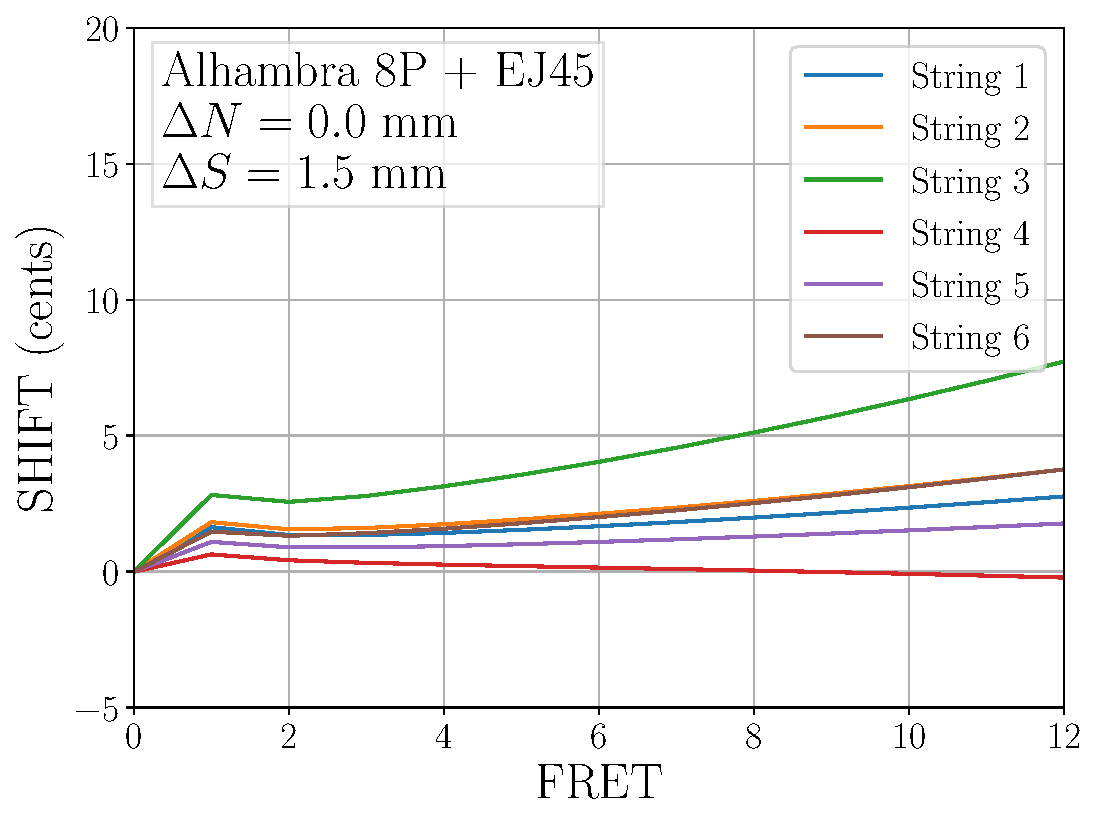
\includegraphics[width=5.0in]{figures/shift_alhambra8p_ej45_factory}
   \caption{Factory guitar}
   \label{fig:shift_alhambra8p_ej45_factory}
  \end{subfigure}
  \par\vspace{0.25in}
  \begin{subfigure}[b]{0.8\textwidth}
   \centering
   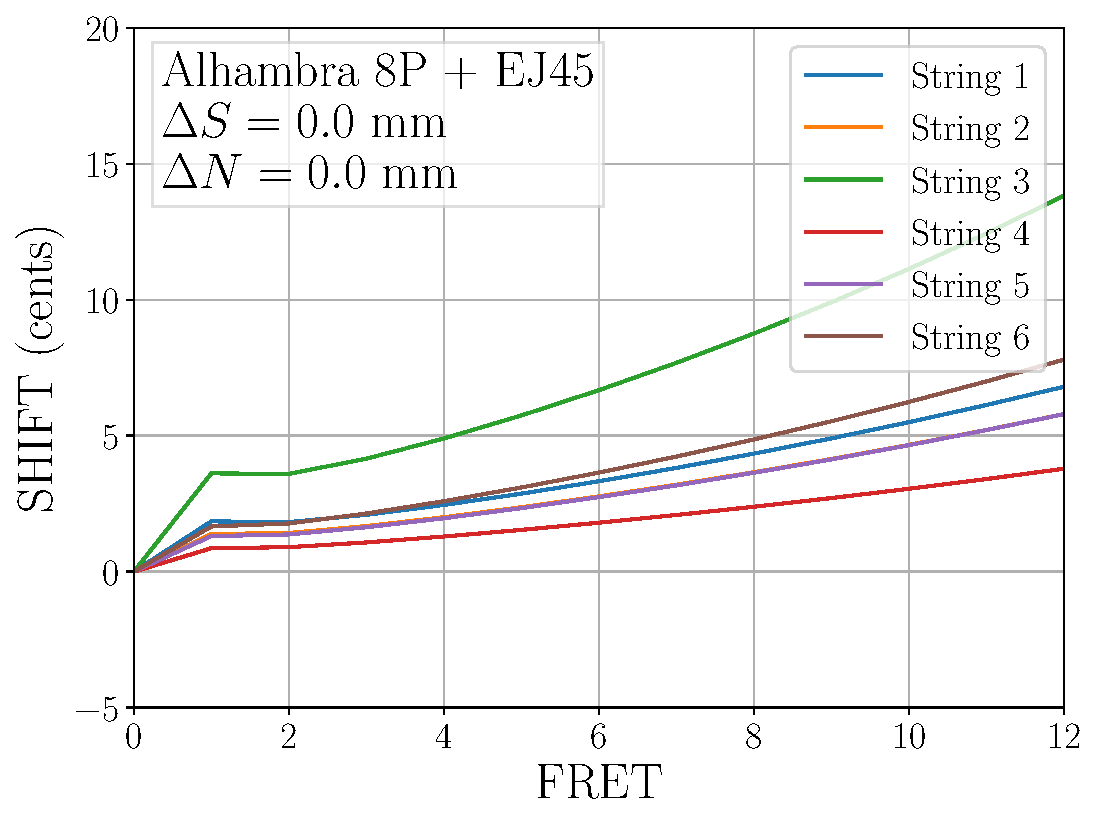
\includegraphics[width=5.0in]{figures/shift_alhambra8p_ej45_null}
   \caption{Uncompensated}
   \label{fig:shift_alhambra8p_ej45_null}
  \end{subfigure}
  \caption{\label{fig:alhambra8p_ej45} Frequency shifts (in cents) for an Alhambra 8P guitar with normal tension nylon strings (D'Addario EJ45). In (a), we show the deviations of the guitar as manufactured in the factory, completely consistent with our measurements. In (b), we show the same 12-TET errors that would arise if $\Delta S = 0$ for the same guitar.}
 \end{figure}

 \begin{table}[htbp]
  \centering
  \caption{\label{tbl:ej45_setbacks} Predicted setbacks for the D'Addario Pro-Arte Nylon Classical Guitar Strings -- Normal Tension (EJ45) on the Alhambra 8P classical guitar.}
  \begin{tabular}{cccc}
\toprule
String &  $\Delta S$ (mm) &  $\Delta N$ (mm) &  $\overline{\Delta \nu}_\text{rms}$ (cents) \\
\midrule
 J4501 &             2.16 &            -0.43 &                                        0.18 \\
 J4502 &             1.92 &            -0.31 &                                        0.15 \\
 J4503 &             4.36 &            -0.82 &                                        0.31 \\
 J4504 &             1.30 &            -0.19 &                                        0.13 \\
 J4505 &             1.94 &            -0.28 &                                        0.15 \\
 J4506 &             2.62 &            -0.35 &                                        0.16 \\
\bottomrule
\end{tabular}


 \end{table}%

 \begin{figure}
  \centering
  \begin{subfigure}[b]{0.8\textwidth}
   \centering
   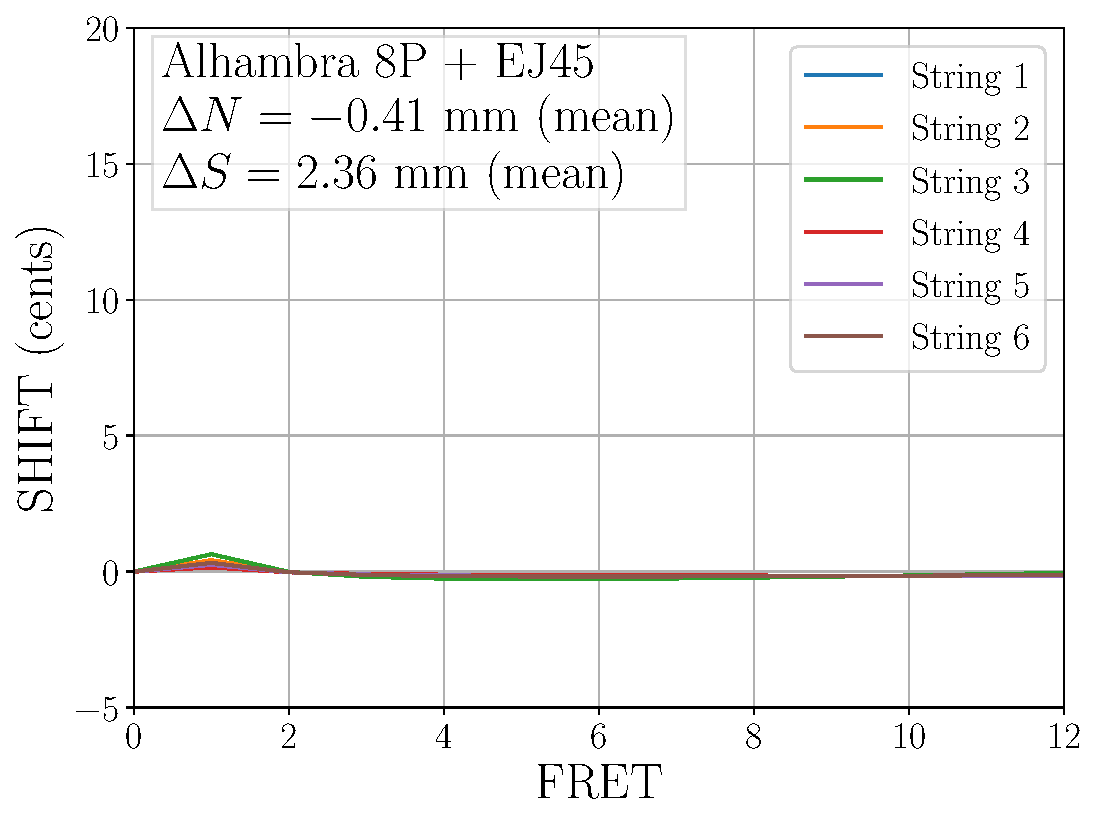
\includegraphics[width=5.0in]{figures/shift_alhambra8p_ej45_full}
   \caption{Full compensation}
   \label{fig:shift_alhambra8p_ej45_full}
  \end{subfigure}
  \par\vspace{0.25in}
  \begin{subfigure}[b]{0.8\textwidth}
   \centering
   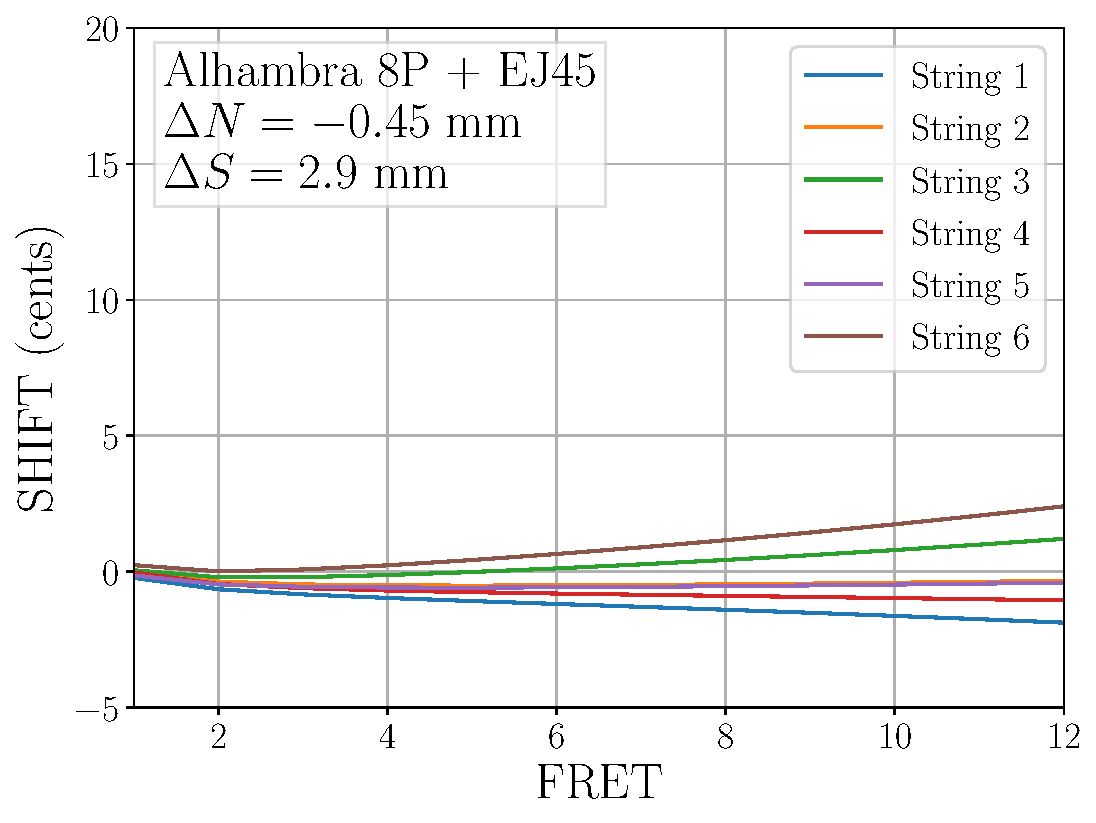
\includegraphics[width=5.0in]{figures/shift_alhambra8p_ej45_mean}
   \caption{Mean compensation}
   \label{fig:shift_alhambra8p_ej45_mean}
  \end{subfigure}
  \caption{\label{fig:compensation_alhambra8p_ej45} Frequency shifts (in cents) for an ``Alhambra 8P'' guitar with normal tension nylon strings (D'Addario EJ45). Instead of the factory setbacks, in (a) we use the individual values for each string that are listed in \tbl{ej45_setbacks}. In (b), we set $\Delta S$ and $\Delta N$ to the mean of the corresponding column in that table.}
 \end{figure}

We close this section with a few comments. First, all of the compensated frequency deviation plots presented in this version of our work are theoretical; in the future, we will present experimental results to determine the efficacy of this compensation approach. Second, it is nontrivial to manufacture a guitar with different setbacks for each string~\cite{ref:byers1996cgi}, and it is unlikely that the exact values listed in \tbl{ej45_setbacks} are applicable to other string sets. We have measured frequency deviations at the 12$^{th}$ fret for three other string sets, and in \app{specs} we have reproduced the compensation procedure for them. There is enough variation in the setbacks across all strings that it would be difficult to find values that could work well for all string sets. Finally, it is possible to simply take the mean setbacks over the all strings in a particular set, and then use these mean values for all strings. We illustrate this approach in \fig{shift_alhambra8p_ej45_mean}; the frequency deviations are not as small as in \fig{shift_alhambra8p_ej45_full}, but they are generally less than 5~cents. In the next section, we discuss a method to temper the guitar to reduce these errors further. 